%%%
 % File:     replay.tex
 % Author:   Hackademics Forum <hackademicsforum6@gmail.com>
 % Project:  MindMap des vulnérabilités
 % Released: 03/08/2016
%%%

%!TeX root = main.tex
%!TeX encoding = UTF-8
%!TeX program = pdflatex
%!TeX spellcheck = fr_FR

%%%
 % Vulnérabilités Replay
%%%
\newpage
\section{Rejeu (Replay / Playback)}\label{vulnerabilites:reseau:replay}

Une attaque par rejeu ou "Replay Attack" est une attaque de type "Man In The Middle". Cette attaque permet à un pirate d'espionner les données échangées entre deux ordinateurs afin de capturer et d'enregistrer des données utiles et confidentielles comme par exemple des informations d'authentification qui pourront ensuite être réutilisées pour être soumises a un ordinateur (client/serveur) ou même a un routeur ,dans le but de faire croire en une connexion légitime. Le pirate pourra ainsi s'authentifier et avoir accès au système en usurpant l'identité de la victime.
\begin{flushleft}
Pour capturer le trafic, le hacker pourra utiliser un script fait maison ou alors plus simplement des logiciels comme wireshark , tcpdump ou zed attack proxy. Ces paquets seront généralement enregistrés au format pcap. Il utilisera ensuite soit à nouveau un script fait maison ou alors un logiciel de type tcpreplay pour renvoyer (rejouer) la séquence afin de se faire passer comme quelqu'un de légitime.
\end{flushleft}

\bigskip

\begin{itemize}
\item Des informations utiles sont envoyées a travers le réseau
\item Un hacker pourra utiliser ces informations afin de les réutiliser a mauvais escient
\item Il aura besoin d'un accès aux données qui se fera
\begin{itemize}
\item Physiquemant
\item Mitm 
\item Malware
\end{itemize}
\item Les informations récupérées seront utiles au pirate
\item Qui pourra les réutiliser en les rejouant pou paraître comme légitime
\end{itemize}

\bigskip

\begin{flushleft}
\textbf{Exemple}
\end{flushleft}

\smallskip

\begin{flushleft}
Supposons une communication entre deux ordinateurs A et B. A va envoyer sa clef à B pour prouver son identité. Mais un pirate C est en train d'espionner cette conversation et décide de garder les informations ainsi obtenues dans la conversation entre A et B. Ces informations lui seront utiles pour se faire passer comme légitime en rejouant les données de connexion à B
\end{flushleft}

\smallskip

\begin{center}
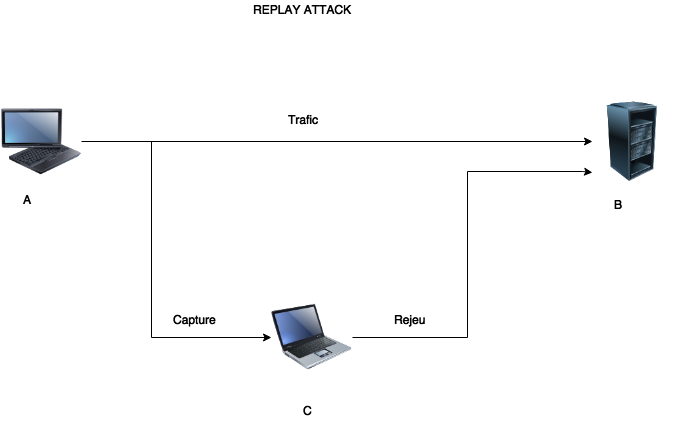
\includegraphics[scale=0.3]{Network/assets/rejeu.png}
\end{center}

\bigskip


\begin{flushleft}
\textbf{Contre-mesures}
\end{flushleft}

\smallskip

\begin{itemize}
\item Un numéro de séquence peut être utilisé. L'authenticité de ce numéro pourra être vérifiée par un code d'authentification de message.
\item L'horodatage est un autre moyen d'empecher les attaques par rejeu. La synchronisation devrait être réalisée en utilisant un protocole sécurisé.
\item L'utilisation de tokens de session uniques en utilisant un processus de génération aléatoire
\item L'utilisation de mots de passe a utilisation unique qui expirent apres un certain temps
\item L'utilisation d'un nombre arbitraire (nonce) a usage unique qui sera utilisé pour signer les echanges de données
\end{itemize}

\bigskip

\begin{flushleft}
\textbf{Lien-utiles}
\end{flushleft}

\begin{itemize}
\item \url{https://www.owasp.org/index.php/Testing_for_WS_Replay_(OWASP-WS-007)}
\item \url{https://www.sitepoint.com/how-to-prevent-replay-attacks-on-your-website/}
\end{itemize}

\endinput
